\documentclass{article}

\usepackage{titlesec}
\titlelabel{\thetitle.\quad}

\usepackage[T1]{fontenc}
\usepackage{inconsolata}

\usepackage[english]{babel}
\usepackage[letterpaper,top=2cm,bottom=2cm,left=2.5cm,right=2.5cm,marginparwidth=1.25cm]{geometry}

\usepackage{hyperref, booktabs, float, listings}
\usepackage[leqno]{amsmath}
\usepackage{enumitem, nccmath,lipsum,amssymb,xcolor,xparse,listings, blindtext}
\usepackage[most]{tcolorbox}

\usepackage{graphicx}
\graphicspath{ {./attachments/} }

\definecolor{light-gray}{gray}{0.9}
\newcommand{\code}[1]{\colorbox{light-gray}{\texttt{#1}}}

\title{Lab 8: Docker}
\author{Mashenkov Timofei B23-CBS-02 \\ \href{mailto:t.mashenkov@innopolis.university}{t.mashenkov@innopolis.university}}
\begin{document}
\maketitle{}

\section{ENTRYPOINT vs CMD}
\noindent

\begin{itemize}
  \item \code{ENTRYPOINT}: used to specify the main command to run when the container starts. Arguments passed to
    \code{docker run} will be appended to it. Use when container is supposed to run as an executable.
  \item \code{CMD}: used to provide default arguments for the \code{ENTRYPOINT} or to specify the main command to run
    when the container starts. Arguments passed to \code{docker run} will override it. Use when container is supposed to
    run as a service.
\end{itemize}

\subsection{Example}
\noindent

\begin{lstlisting}
  ENTRYPOINT ["python3"]
  CMD ["-m", "http.server", "8000"]
\end{lstlisting}

\begin{itemize}
  \item \code{docker run myimage} → \code{python3 -m http.server 8000}
  \item \code{docker run myimage app.py} → \code{python3 app.py}
\end{itemize}

\section{Security precautions}
\noindent

\begin{enumerate}
  \item Keep both host and Docker up-to-date
  \item Run containers as non-root user
  \item Limit container capabilities: \code{--cap-drop=all}
  \item Use trusted images
  \item Apply resource limits: \code{--memory=100m}
\end{enumerate}

\section{Remove All Exited Containers}
\noindent

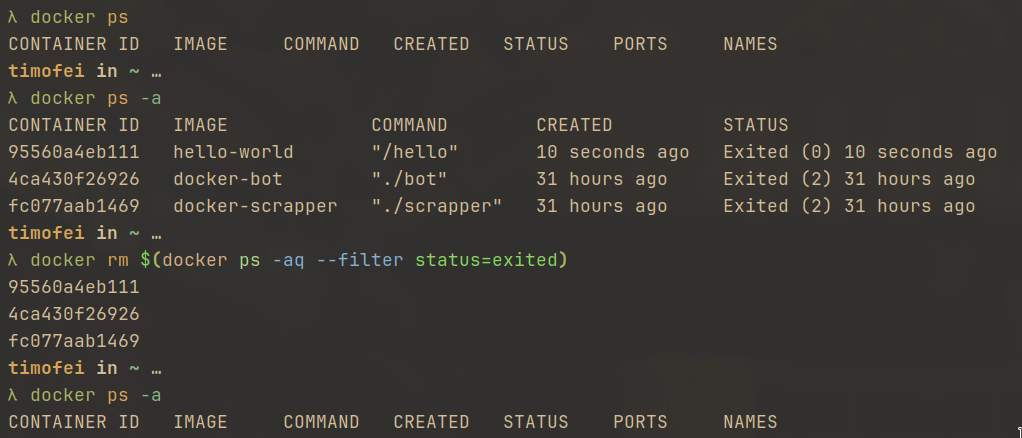
\includegraphics[width=480pt]{remove_exited_containers.jpg}

\section{Copy Files to Running Container}
\noindent

Simply using command \code{docker cp /path/on/host.txt container\_name:/path/in/container/}.

\subsection{Example}
\noindent

\code{docker cp index.html ngingx-web:/usr/share/nginx/html/}. 

\newpage
\section{Dockerized Nginx}
\noindent

The following example demonstrates how container takes in modified \code{index.html} file.

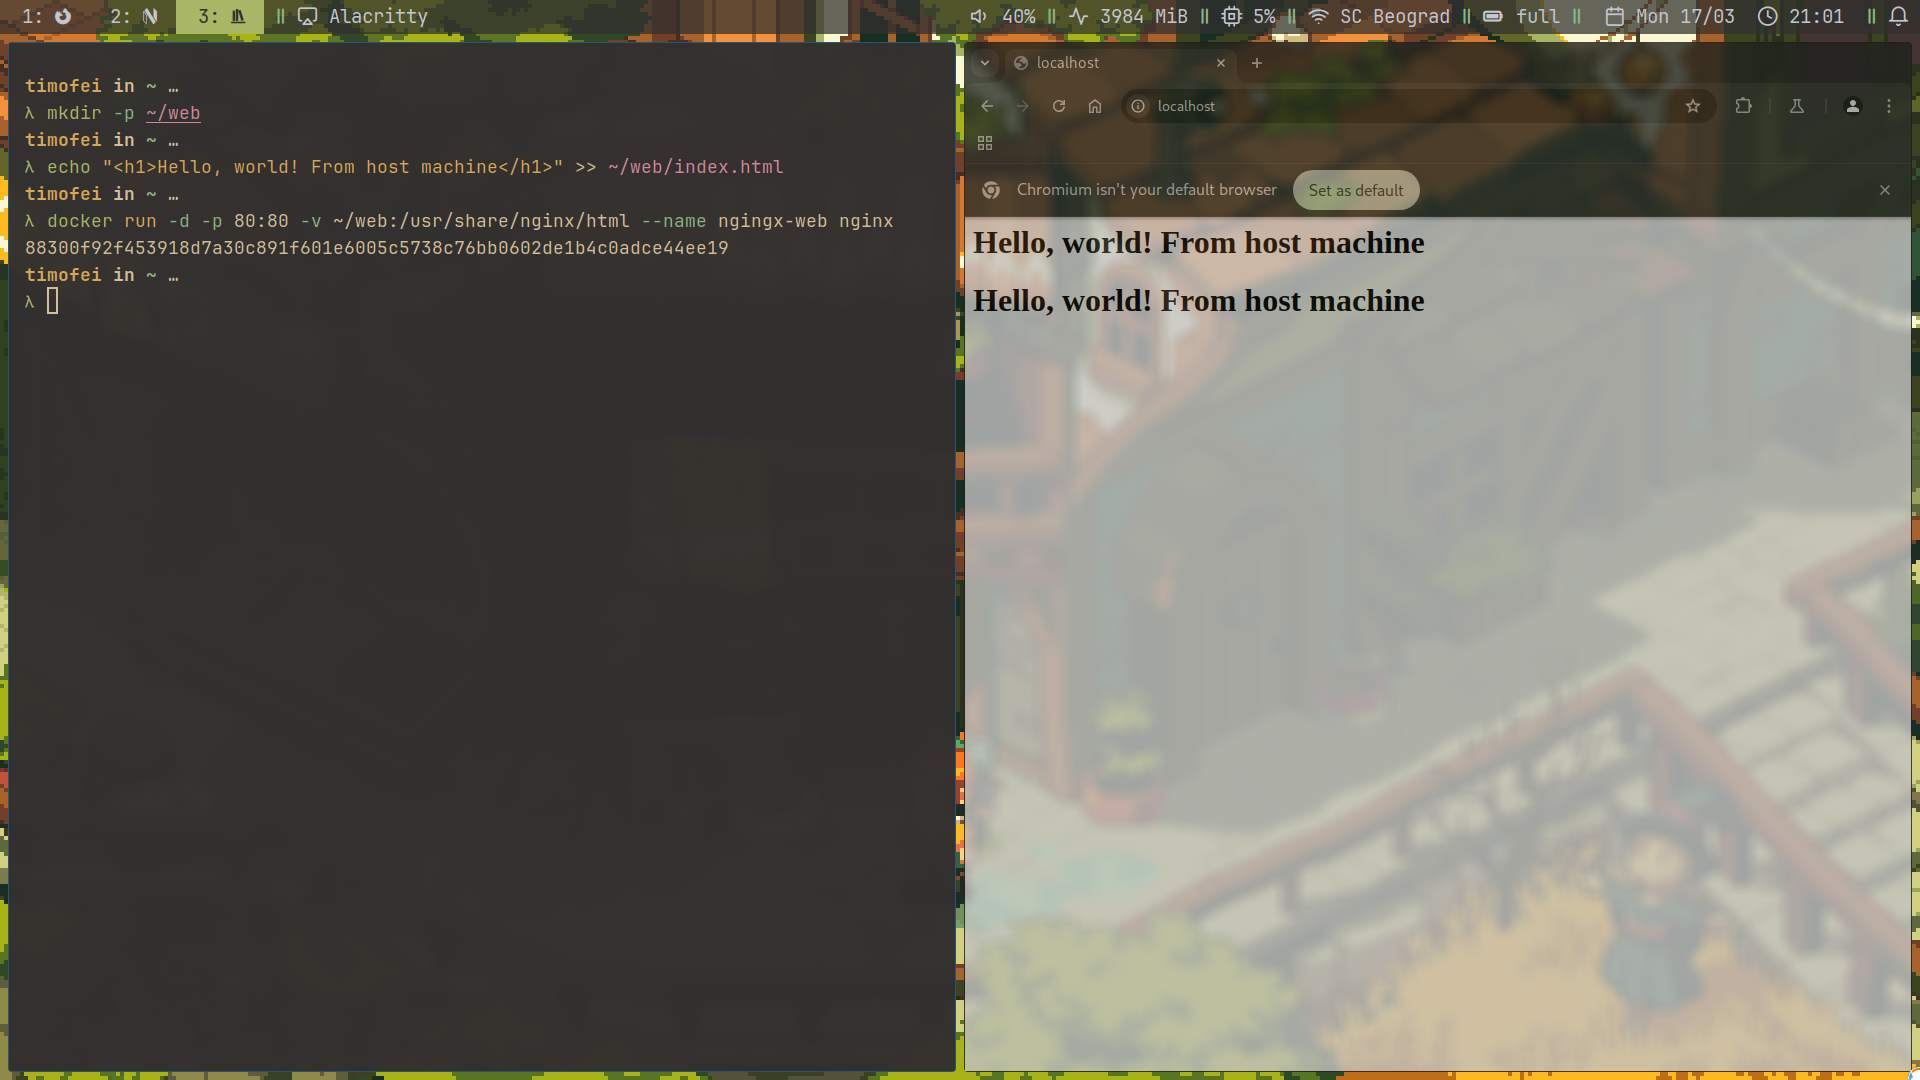
\includegraphics[width=480pt]{nginx_before.jpg}

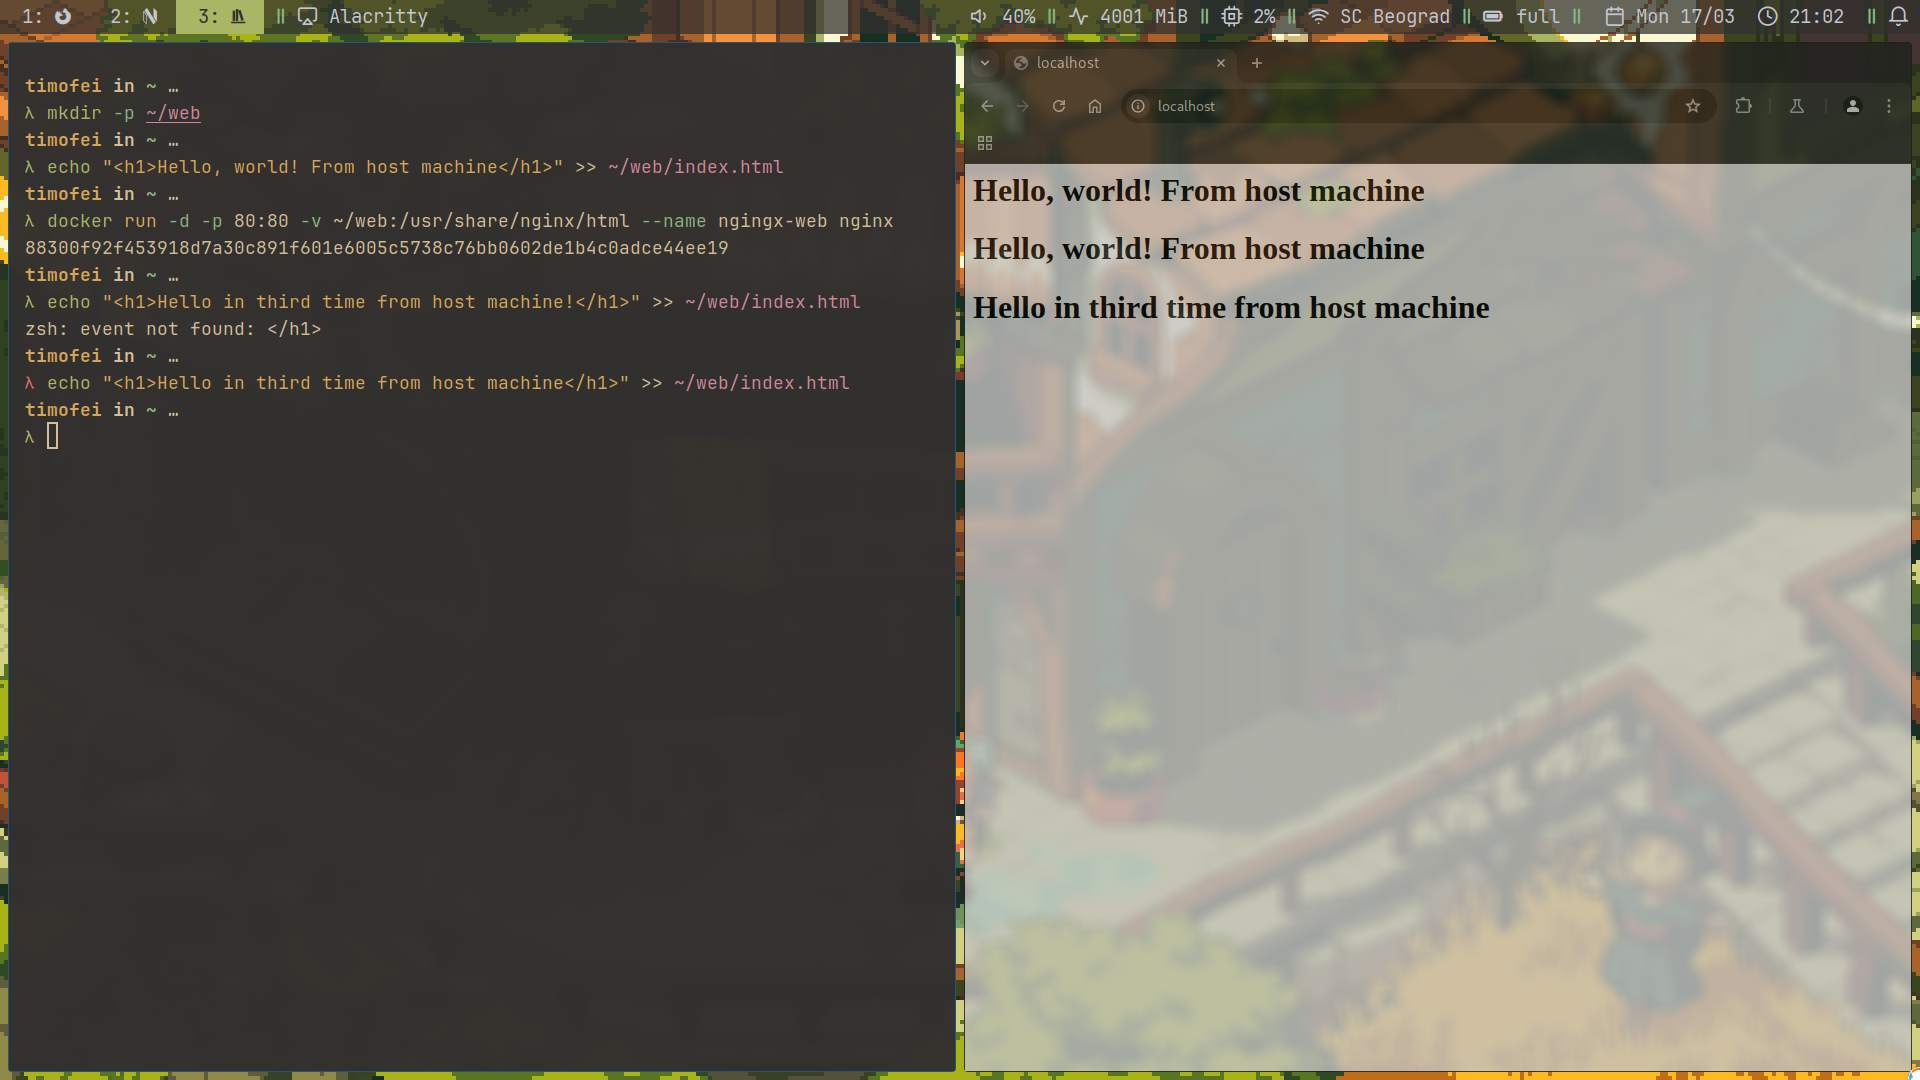
\includegraphics[width=480pt]{nginx_after.jpg}

\section{Logging with Rsyslog}
\noindent

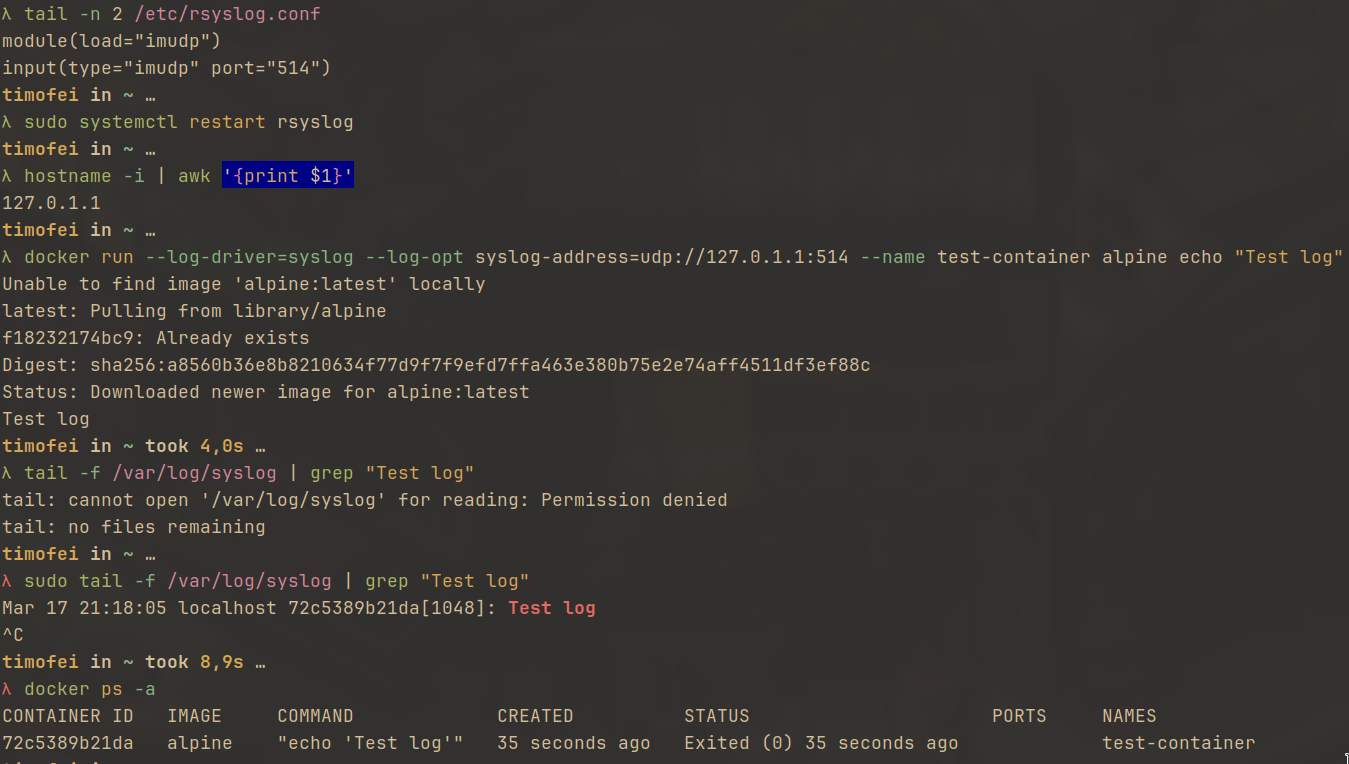
\includegraphics[width=480pt]{rsyslog.jpg}
\noindent

\subsection{Steps to reproduce}

\begin{enumerate}
  \item Install \code{rsyslog} on the host machine, then configure it to listen on port 514.
  \item Restart \code{rsyslog} service.
  \item Find out host machine IP
  \item Run container specifying log driver as \code{syslog} and \code{syslog-address} as \code{<protocol>://<host\_ip>:514}.
  \item Check logs on the host machine.
\end{enumerate}

Example shows that log message belongs exactly to the container since it contains container ID.

\section{Docker Hub}
\noindent

I already have one! Do not really know what is there, but \href{https://hub.docker.com/repository/docker/mashfeii/catnip/}{here is the link}


\newpage
\section{Bonus: Dockerfile Fix}
\noindent

\begin{itemize}
  \item \code{apk} instead of \code{apt-get}
  \item \code{python3} instead of \code{python}
  \item \code{>} instead of \code{>>}
\end{itemize}

\begin{figure}[h]
  \centering

  \caption{Steps to create fixed Dockerfile}
  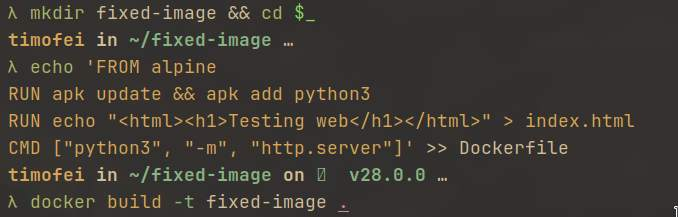
\includegraphics[width=480pt]{dockerfix_image.jpg}

  \caption{Steps to run image and check the result}
  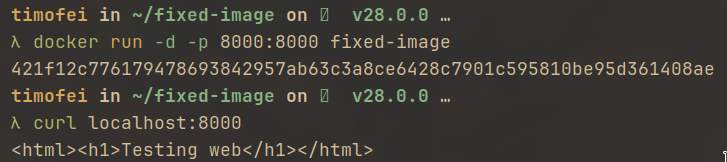
\includegraphics[width=480pt]{dockerfix_test.jpg}
\end{figure}

\end{document}
